\subsection{Geofeedia}

Geofeedia \cite{geofeedia} es un servicio pionero en el control de origen de los medios de comunicación social mediante geolocalización, permite monitorear y  realizar análisis a datos provenientes de las redes sociales, complementando la tradicional búsqueda de \emph{keywords} que típicamente pierden información sobre la actividad social relacionada, ayudando a reducir el desorden de los medios sociales en tiempo real. Geofeedia realiza búsquedas en las redes sociales: Twitter, Instagram, YouTube, Picasa, y Flickr. Posee una interfaz intuitiva y fácil de usar además de un conjunto de herramientas para facilitar las búsquedas. Geofeedia permite obtener stream de datos de redes sociales provenientes de una zona geográfica en específico, mediante la mención textual del lugar o la delimitación de una región en un mapa interactivo.

Los diversos feeds se pueden categorizar y "olvidar" usuarios (no recibir feed de dicho usuario). Los resultados de la búsqueda se pueden filtrar por fecha, por palabras claves, por tipo de medio social y por autor, entre muchos otros. La plataforma además permite variadas herramientas de análisis como identificar la tendencia de palabras claves, la actividad basada en el tiempo, frases influyentes, las fuentes de los medios sociales y exportar a través de la API en formatos CSV ATOM, GeoRSS, JSON, KML.

\begin{figure}[H]
	\centering
	\begin{minipage}[t]{.45\textwidth}
		\begin{center}
			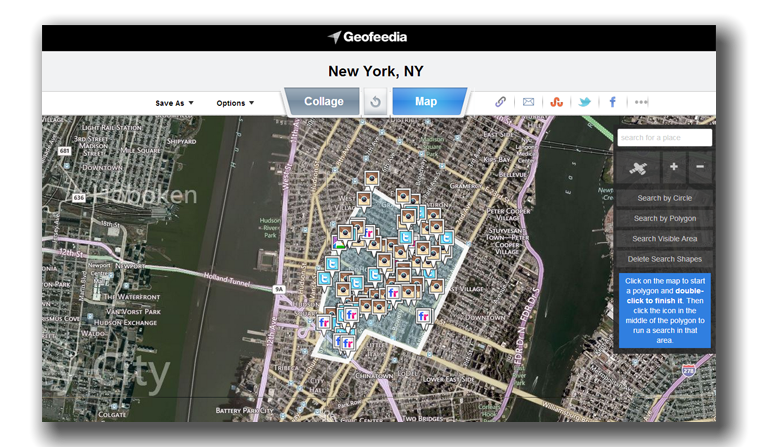
\epsfig{file=imgs/geofeedia1.png, width=2.5in} 
			  \caption{Imagen del mapa interactivo de geofeedia donde en una zona delimitada por el usuario se reciben todos los feeds de los medios sociales.}
			  \label{fig:geofeedia1}
		\end{center}
	\end{minipage}
	\hfill
	\begin{minipage}[t]{.45\textwidth}
		\begin{center}
			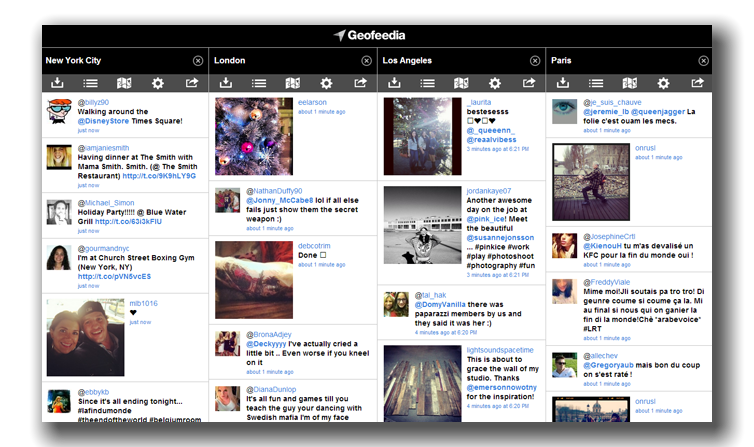
\epsfig{file=imgs/geofeedia2.png, width=2.5in} 
			\caption{Imagen del panel de noticias de geofeedia, donde cada columna recoge los feeds para ubicaciones geográficas distintas.}
			\label{fig:geofeedia2}
		\end{center}
	\end{minipage}
	\hfill
\end{figure}

\subsection{Paper.li}\label{subsec:paperli}

Paper.li \cite{paperli} es una creación de la startup suiza Small-Rivers con sede en Lausanne. Es una herramienta que permite generar una especie de periódico personalizado en base a las publicaciones en redes sociales de los contactos (en dichas redes) del usuario. Actualmente Paper.li permite el acceso a fuentes como Twitter, Facebook, Google, YouTube y los canales RSS para la recolección de información, permitiendo fáciles combinaciones de las distintas fuentes de contenido, la priorización temática, la aplicación de filtros de contenidos y la configuración las fuentes de información.

El funcionamiento de Paper.li se basa en el hecho de que muchas usuarias y usuarios de Twitter confían más en el criterio de selección de sus redes sociales para identificar enlaces a noticias importantes que en las compilaciones que realizan los diarios tradicionales. Paper.li recoge los enlaces a noticias, fotos y vídeos de una cuenta en Twitter y otras redes sociales;  realiza una selección de estos vínculos (a partir de un análisis realizado con “herramientas de análisis semántico de texto”), crea una página diaria editada con aspecto a una página de los periódicos tradicionales que vemos en Internet, donde los enlaces y el contenido aparecen divididos en secciones contextuales.

%Los creadores de Paper.li (mediante el blog oficial del medio) han declarado que la motivación inicial para crear este medio “no es por la sobrecarga de información es por la ausencia de un filtro“. 
Es importante señalar que Paper.li no cumple exactamente con la tarea de entregar las noticias de forma urgente debido a su intervalo de actualización diario, Paper.li más bien, reporta el eco de las noticias en las redes sociales: la reproducción de contenidos más frecuentes, los tópicos más consultados o lo más recomendados.

\begin{figure}[H]
	\centering
	\begin{minipage}[t]{.45\textwidth}
		\begin{center}
			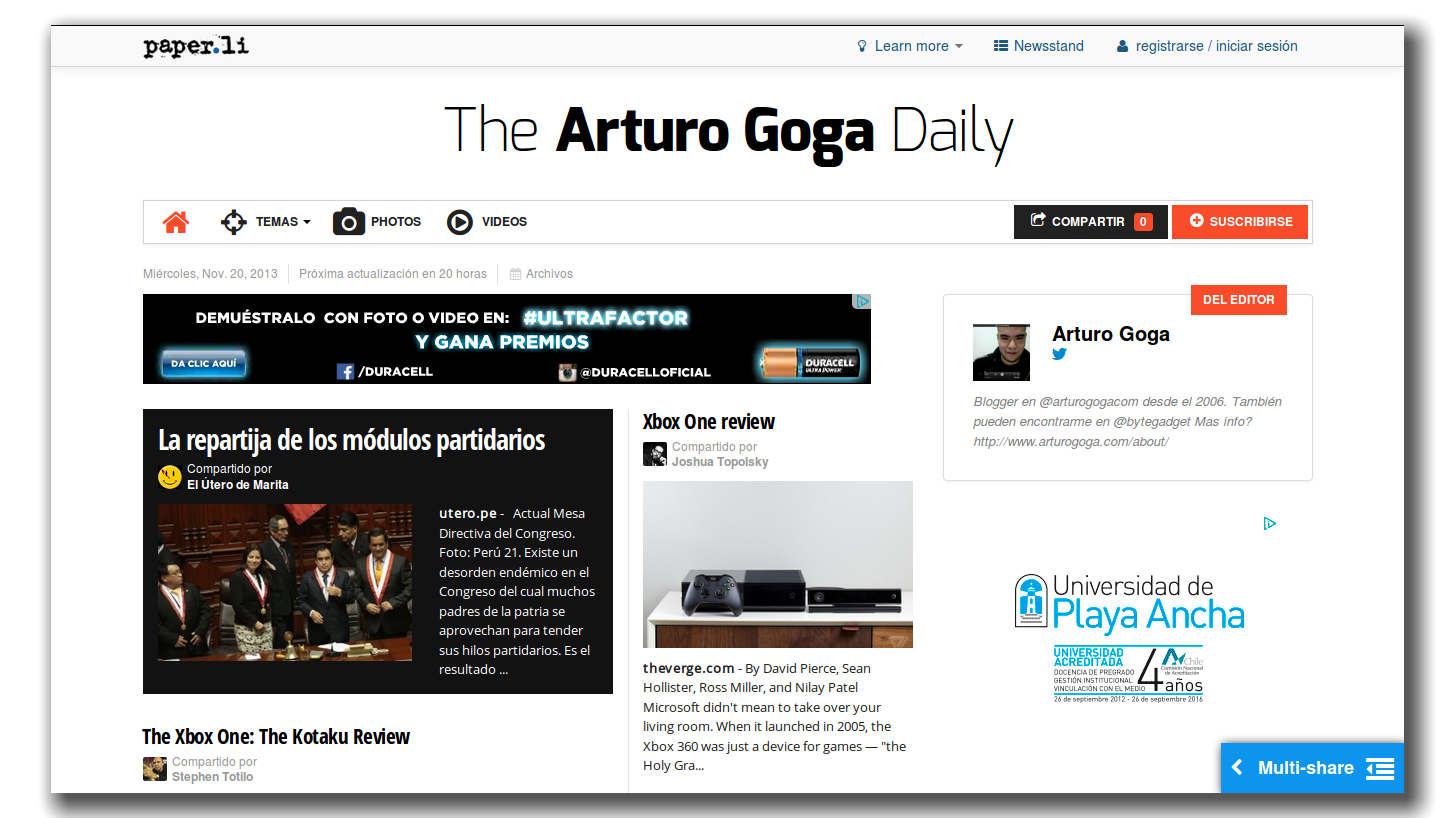
\epsfig{file=imgs/paperli1.png, width=2.5in} 
			\caption{Vista principal del periodico Paper.li de un usuario de la plataforma}
			\label{fig:paperli1}
		\end{center}
	\end{minipage}
	\hfill
	\begin{minipage}[t]{.45\textwidth}
		\begin{center}
			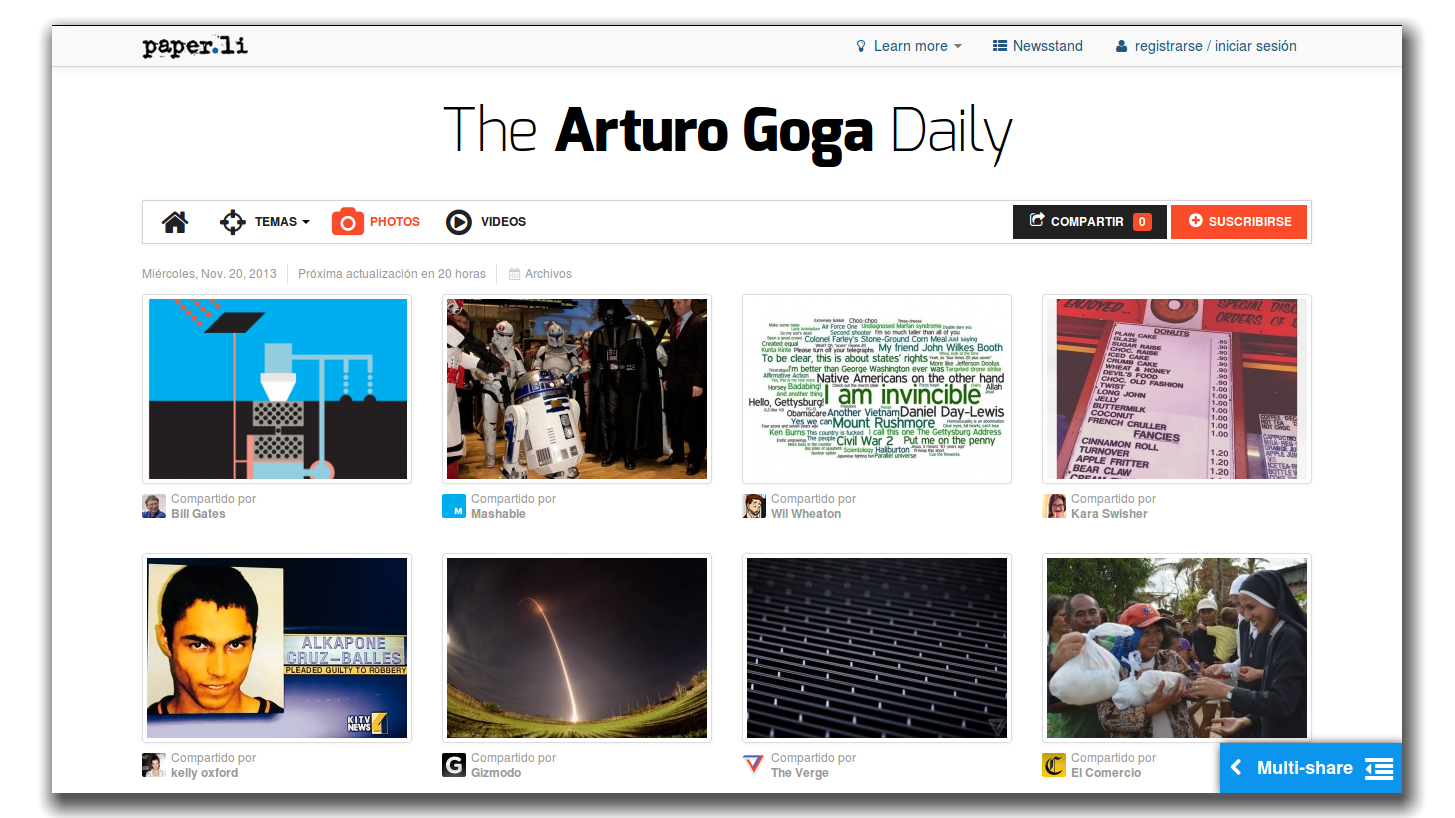
\epsfig{file=imgs/paperli2.png, width=2.5in} 
			\caption{Vista de fotografías del periodico Paper.li de un usuario de la plataforma}
			\label{fig:paperli2}
		\end{center}
	\end{minipage}
	\hfill
\end{figure}


\subsection{The Tweeted Times}

The Tweeted Times \cite{tweetedtimes} es una aplicación web lanzada en 2010 y desarrollada por Flipboard, Inc. permite generar en base a los \emph{feeds} recibidos en la cuenta de Twitter, una especie de periódico de noticias con las temáticas más importantes, de forma similar a Paper.li \ref{subsec:paperli} pero sólo enfocado en Twitter y con la potencialidad de que se actualiza cada una hora.

The Tweeted Times posee otras potencialidades como su capacidad de personalización en la selección de los contenidos. Además de la cuenta del mismo usuario, es posible crear periódicos con listas particulares de Twitter, con perfiles de usuarios, y hasta de una búsqueda de un hashtag o de usuarios, además de permitir explorar los periódicos de otros contactos en Twitter y de usuarios destacados de la plataforma. Para la organización de las publicaciones de acuerdo a su relevancia el algoritmo utilizado se basa principalmente en la repercusión de dichas publicaciones en Twitter (cantidad de re-tweet y número de favoritos).  

\begin{figure}[H]
	\centering
	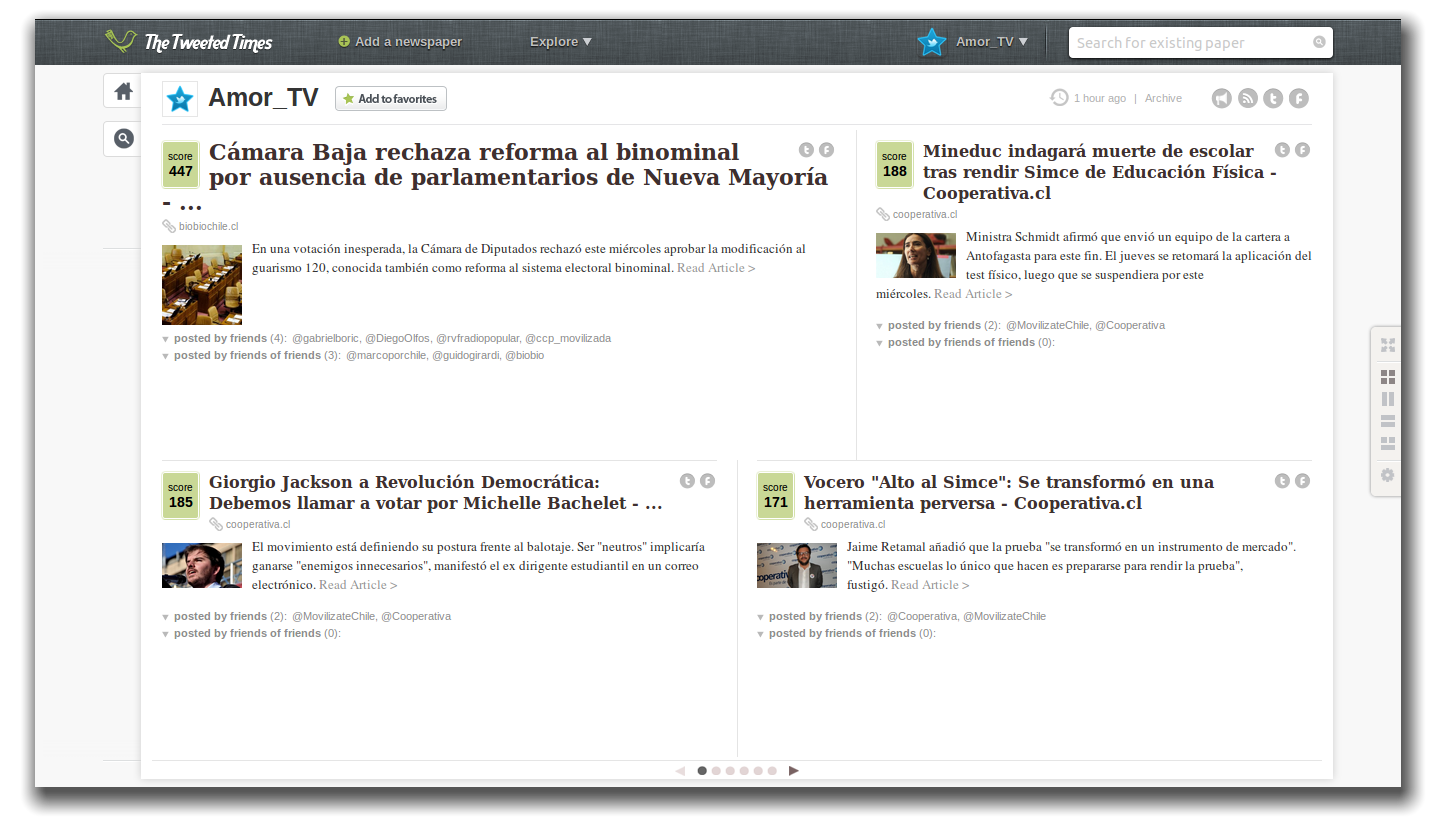
\includegraphics[width=0.8\textwidth]{imgs/tweettimes.png}
	\caption{Vista principal de un periodico creado en The Tweeted Times}
	\label{fig:tweetedTime}
\end{figure}

\subsection{FlipBoard}

Flipboard \cite{flipboard} es una aplicación lanzada en julio de 2010 que permite reunir las noticias del mundo y las novedades de las redes sociales en una revista diseñada para dispositivos móviles. El usuario puede elegir algunas temáticas y Flipboard crea una revista digital, en la cual se pueden ``hojear" las noticias de interés, historias y fotos que los contactos del usuario compartan. Flipboard posee además una función que permite guardar artículos para verlos posteriormente o recopilarlos en ``revistas" propias de Flipboard.

%Flipboard promociona sus pontencialidades de la siguiente manera: ``Muévete a través de las noticias desde tu Twitter y publicaciones como la BBC, USA Today y The Verge. Entérate de todo, desde las fotos y mensajes compartidos por tus amigos en Facebook e Instagram, hasta los videos de YouTube y las novedades de la cultura pop de la revista Rolling Stone. Encuentra inspiración para tus viajes, moda y vida en sitios como la National Geographic, Elle España, Oprah y Cool Hunting. O crea tus propias revistas sobre cualquier tema, desde culinaria hasta Química". 
%https://play.google.com/store/apps/details?id=flipboard.app&hl=es_419

Actualmente permite la conexión con 12 redes sociales entre las que se incluyen Twitter, Facebook, Instagram, Google+, YouTube, Google Reader, LinkedIn, Flickr, 500px, Sina Weibo y Renren, en las cuales es posible realizar búsquedas mediante temas, hashtag, blogs y personas. Hoy en día existen 15 diferentes versiones de Flipboard entre países de América, Europa y Asia. Flipboard también pone a disposición de sus usuarios y usuarias contenidos seleccionados donde se incluyen las revistas y blog recomendados, fotografías y secciones especiales a noticias del día y temas de interés.

\begin{figure}[H]
	\centering
	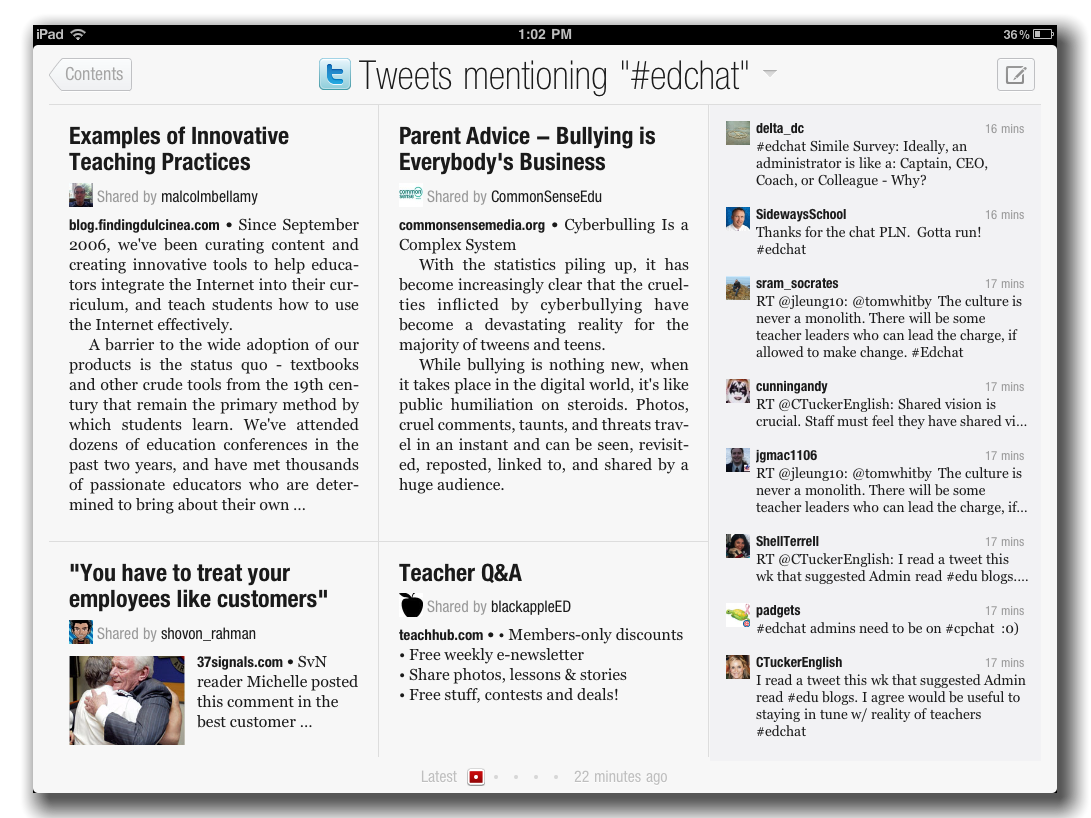
\includegraphics[width=0.8\textwidth]{imgs/flipboard3.PNG}
	\caption{Vista del formato de revista en Flipboard para visualizar los feeds de Twitter, donde se resaltan los tweet que han tenido mayor repercusión en la red y los enlaces compartidos}
	\label{fig:flipboard1}
\end{figure}

\subsection{Summify}

Summify\cite{summify} consistía en un servicio gratuito que permitía informarse de la actualidad por medio de recopilaciones diarias de las noticias que más circulaban entre el círculo de contactos de Twitter, Facebook, Google Reader o feeds RSS del usuario. Summify cesó sus funciones el 22 de junio de 2012 por decisión de Twitter a solo cinco meses de comprarlo. Summify entregaba su servicio de distintas formas: mediante la web para revisar las recopilaciones, vía correo electrónico, mediante la notificación por DM de Twitter cuando existe una nueva disponible y mediante la aplicación móvil.

La principal motivación para esta aplicación se refiere a lo costoso en tiempo que es mantenerse informado en las redes sociales \footnote{"...En un inicio mantenerse al tanto de las actividades sociales es muy gratificante, pero luego, fácilmente, se puede convertir en una actividad agobiante y poco productiva por la gran cantidad de contactos y las diversas redes sociales existentes \cite{summifyvideo}."}. Summify se presentaba como una alternativa productiva para mantener satisfactoriamente los vinculos sociales en la red.

Summify permitía la configuración de la cantidad de recopilaciones que se deseaba recibir el usuario (de una a cuatro diarias) y la hora de recopilación de la primera de éstas (las restantes se realizaban en consecusión en horas), era posible especificar la cantidad de artículos que poseían dichas recopilaciones (de dos a quince artículos), además de su privacidad (públicas o privadas). Su algoritmo se encargaba de recopilar los enlaces a artículos que aparecen en las cuentas del usuario en Twitter y Facebook y los filtraba según su impacto ( cantidad de veces compartido, cantidad de “Me gusta” o cantidad de re-tweeteados), prestando atención a las personas con las que el usuario interactua más. 

El algoritmo consideraba también el impacto a nivel global pero con menor consideración que las recomendaciones de los contactos \cite{summifyblog}. Otra cualidad del algoritmo es la capacidad de aprender en base al uso dado por la o el usuario, analizando las tendencias y preferencias de uso, observando si se pinchaban más historias de un usuario en particular, en un dominio concreto, si contienen palabras claves dentro del título o según la fuente de feeds más utilizada. Cada recopilación poseía su propia página individual y mostraba las noticias seleccionadas una debajo de la otra. Junto a ellas, se visualizaban algunos de las y los usuarios que las habían compartido y al posicionar el puntero por encima de los avatares, el mensaje en el cual compartieron el artículo.

En el caso de que algunos de los contactos del usuario en Twitter y Facebook también estén usando Summify, era posible acceder a sus recopilaciones (en el caso de que éstas fuesen públicas). Era posible también navegar por los perfiles y recopilaciones de los usuarios que se siguen, que siguen al propio usuario y, además, de los que se considera que influencian al usuario y a los que influencian al usuario (es decir, que aparecen más veces en los resúmenes del usuario o en los que aparecemos más veces el propio usuario).

\begin{figure}[H]
  \centering
    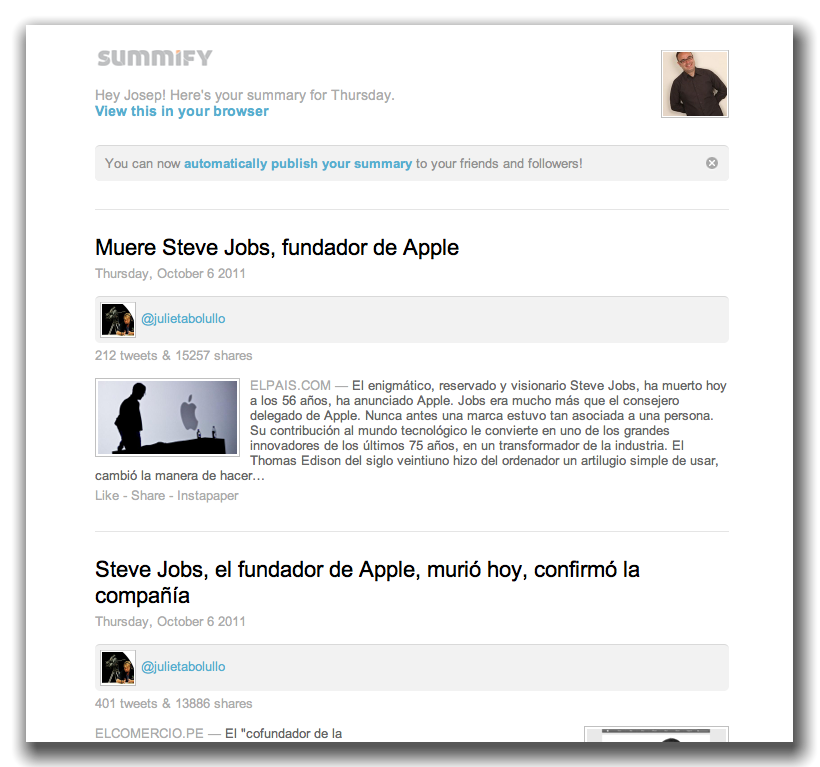
\includegraphics[width=0.8\textwidth]{imgs/summify.png}
  \caption{Vista de la recopilación de Summify}
  \label{fig:summify}
\end{figure}

\subsection{TwitterFall}

Twitterfall \cite{twitterfall} es un cliente web para Twitter que permite realizar búsquedas avanzadas y seguimiento de temas de tendencia. Fue construida el 2009 por Tom Brearley y David Somers, dos estudiantes de ciencias de la computación de 19 años en la Universidad de York y después de tres años de funcionamiento ha sido denominado como ``el google para la tweet-osfera". El nombre de la plataforma se relaciona con la forma de su interfaz, ya que se presenta como una cascada de tweets. éstos caen (hacia abajo de la pantalla) a medida que existen nuevas actualizaciones en tiempo real. La velocidad de este flujo puede ser personalizada mediante un simple ajuste.

Las potencialidades de TwitterFall radican en sus herramientas de búsqueda, entre las cuales se encuentran:
\begin{itemize}
	\item Realizar búsquedas mediante palabras claves o trending topic.
	\item Realizar búsquedas geolocalizadas.
	\item Realizar filtrados por idioma y excluir re-tweet.
	\item Almacenar las búsquedas favoritas.
\end{itemize}

TwitterFall permite también iniciar sesión en Twitter desde su interfaz y utilizarlo como cliente regular de Twitter para responder mensajes, realizar re-tweet, seguir a nuevas personas, etc. otorga además interesantes características como pre-visualizaciones en ventanas flotantes sobre enlaces contenidos en tweets (sin necesidad de ser redirido a ellos)

%sobre un tweet se obtiene información sobre su ubicación y sus seguidores.

%TwitterFall también permite una gran cantidad de opcionees de presentación, como la personalización del tamaño de la fuente, el color, acelerar o disminuir la velocidad de refresco de la cascada de tweets. 

\begin{figure}[H]
	\centering
	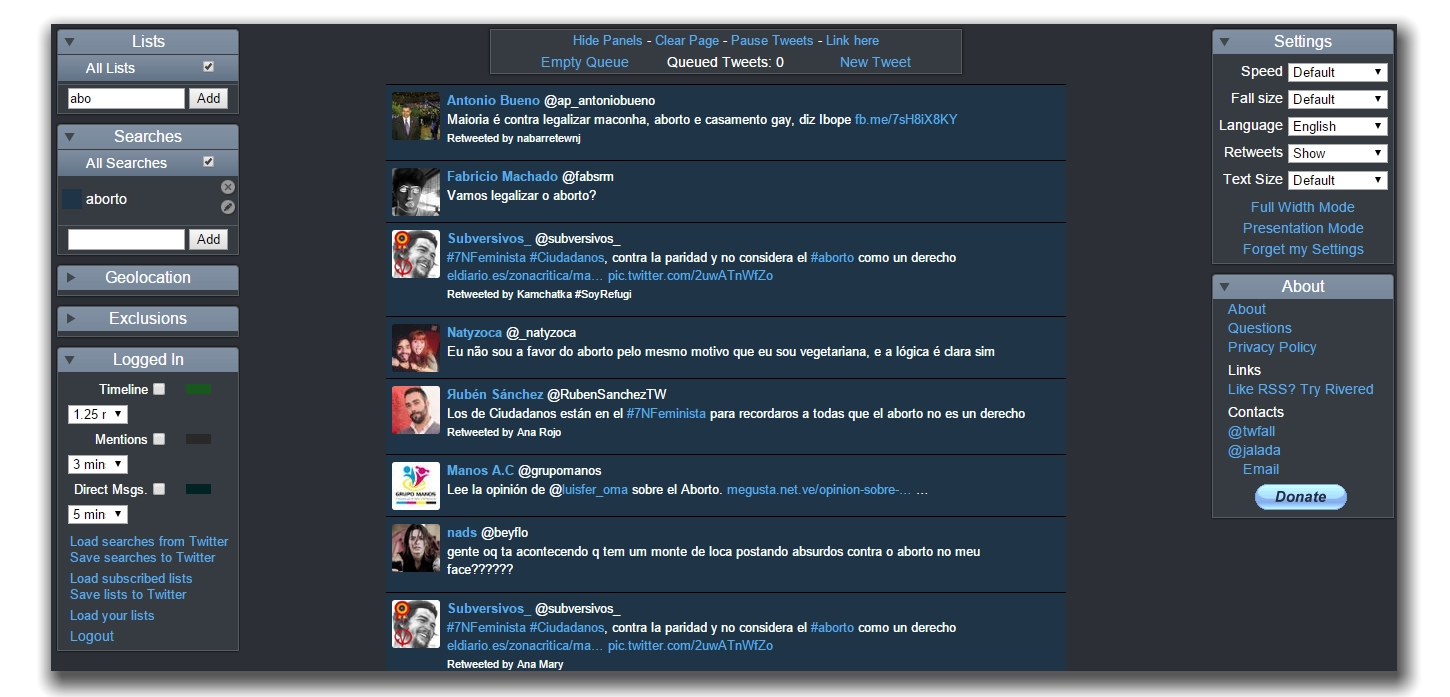
\includegraphics[width=0.8\textwidth]{imgs/twitterfall.jpg}
	\caption{Vista de la recopilación de Twitterfall}
	\label{fig:twitterfall}
\end{figure}

\subsection{Storyful}

Fundada en Dublín con sólo tres empleados, Storyful \cite{storyful} tiene su razón de ser en idear una manera de administrar las enormes cantidades de contenido que se comparten en las redes sociales, aplicando procesos y tecnología eficaz para ayudar a filtrar ``noticias de ruido". Storyful pretende dotar de herramientas a todos los medios de prensa que las demanden \footnote{ Tal como declaran en su página web: "Desde 2010, Storyful ha estado construyendo y perfeccionando la primera sala de prensa verdaderamente social. Hemos perfeccionado nuestras técnicas, herramientas y servicios, en colaboración con algunas de las marcas más importantes de noticias en el mundo, incluyendo ABC News, Reuters y el New York Times, y plataformas sociales como YouTube." }.

%Definiendo su servicio como ``Storyful es la primera agencia de noticias de la era de los medios sociales. Ayudamos a las salas de redacción a encontrar el contenido más valioso en la web social." \footnote{\url{http://storyful.com/about/}}. 

%A finales del 2011 Storyful formó una alianza con YouTube para encontrar y la validar los vídeos que surgieron a partir de las protestas crecientes en Egipto.
Storyful ha desarrollado lo que llaman como ``algoritmo humano" que consiste en un conjunto de procesos algorítmicos y humanos que posee gran aceptación hoy en el mercado de las noticias obtenidas de medios sociales. 
%uestra ambición es ayudar a cada organización de noticias a construir su propia sala de redacción social. Queremos equipar a todos los periodistas con las habilidades y herramientas necesarias para aceptar el cambio. Queremos ayudar a los editores y locutores construir productos que realizan las audiencias y ganar dinero. "

Storyful plantea que las y los periodistas deben pensar en su papel en un mundo cambiante, comenzando a utilizar nuevas herramientas inteligentes y rápidas, complementándolas con los conocimientos profesionales y de oficio de los periodistas. Separando el proceso en tres etapas: descubrimiento de hechos noticiosos, verificación y entrega o presentación de los contenidos. Aseguran que la única manera de verificar una información y restringir correctamente su ruido es unirse a la conversación sostenida en los medios sociales desde donde surgen los hechos noticiosos,  pero no sólo escuchar en ellos, sino participando directamente, de forma abierta y honesta con las voces más cercanamente relacionadas con el hecho \footnote{Tal como indican en su bloh: "La mayoría de las organizaciones de noticias se busque en observadores pasivos. Pero eso no es suficiente. La única manera de desbloquear el poder de la Algoritmo humano es ser una parte de ella" \url{http://storyful.com/about/}}.

Señalan que el valor de la información al relacionarse en los grupos de redes sociales es increíble, apasionante y de rápida evolución, pudiendo explicitar relaciones con otros hechos noticios aparentemente invisibles, que finalmente enriquecen la noticia y la completan, permitiendo contacto y conversaciones abiertas, informadas y sinceras con los lugareños del mismo sector o con acádemicos de la zona, con información que de otro modo dificilmente fuese recolectada. Storyful plantea que fue diseñado para ``vivir dentro de las comunidades de medios sociales, no para observar desde una distancia segura". Para lo cual cuenta con jueces en terreno que establecen vínculos sociales y contactos con personas del entorno para acreditar desde estas relaciones, la veracidad de la información, complementando el proceso de verificación establecido para un hecho en específico.

\begin{figure}[H]
	\centering
	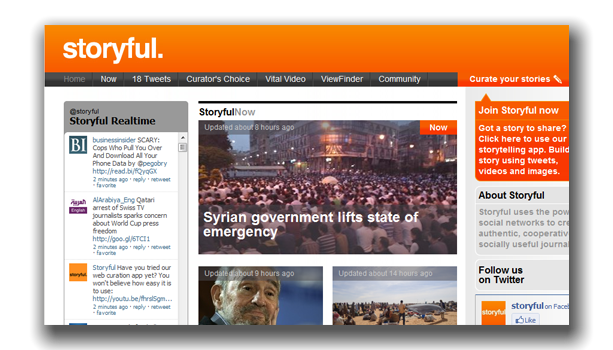
\includegraphics[width=0.8\textwidth]{imgs/storyful.png}
	\caption{Vista principal de Storyful}
	\label{fig:storyful}
\end{figure}

%El proceso de verificación es la piedra angular del proceso, puesto que muchas veces en las redes sociales se hacen circular deliberadamente informaciones incorrectas, generando desinformación y percepciones erradas. En dicho proceso aplican las siguientes preguntas para generar un cierto nivel de fidelidad de la información aportada por un cargador en Youtube:

%\begin{itemize}
%	\item ¿Dónde se ha registrado esta cuenta y en que se ha basado el autor para emitir su juicio de la historia?
%	\item ¿Existen otras cuentas en Twitter, Facebook, blogs o sitios web relacionados a este autor ? ¿Qué información tienen para indicar la ubicación reciente, la actividad, la fiabilidad y/o el sesgo?
%	\item ¿Hace cuánto tiempo existen esas cuentas? ¿Qué tan activas son?
%	\item ¿La narración del contenido se escribe en jerga o dialecto identificable en la narración de la publicación?.
%	\item ¿Podemos encontrar información WHOIS\footnote{Es un protocolo de petición y respuesta ampliamente utilizado en bases de datos para el registro de usuarios o asignaciones de algun recurso de Internet, como el nombre del dominio o el bloque de dirección IP} para algún sitio web afiliado ?
%	\item ¿El cargador aparece en los directorios locales ? ¿Qué indican sus círculos sociales en línea que están cerca de esta historia / ubicación?
%	\item ¿Tiende el cargador a "copiar" contenidos de otras cuentas de Youtube o carga únicamente contenido generado por el usuario?
%	\item ¿Los vídeos de la cuenta del cargador tienen una calidad consistente?
%	\item ¿La descripción del vídeo es consistente y señalan un lugar específico ? ¿Corresponde la fecha? ¿Tiene la extensión de archivo como AVI o MP4 en el título del video?
%	\item ¿Storyful esta familiarizado con esta cuenta? ¿su contenido ha sido fiable en el pasado?
%\end{itemize}

%Storyful comparte sus conocimientos y técnicas de forma abierta desde el blog.
% de su plataforma los cuales se revisan a continuación debido a su posible aplicabilidad como directrices en este trabajo:

%\begin{itemize}
%	\item{\textbf{Hacer listas: Cómo afinar sus antenas Twitter}} \cite{storyfulblog}
	
	%Una herramienta fundamental para el funcionamiento de Storyful, son las listas temáticas de Twitter. Debido al amplio flujo de información en la era de los medios sociales, las listas funcionan como el filtro perfecto de noticias en vivo, permitiendo afinar el lugar de observación, un objeto o un evento y silenciar algunas conversaciones no útiles que tienen lugar simultáneamente.
	
	%Manejan simultáneamente cientos de listas de Twitter que cubren todos los países del mundo y todos los temas imaginables es complejo. 
	
	%Para la administración de estas listas se utiliza la herramienta \emph{Tweetdeck}\cite{tweetdeck}, donde a cada terminal se le cargan cerca de 20 a 30 listas para ser visualizadas por un periodista. \emph{Tweetdeck} es utilizado (a pesar de sus limitantes en el número de listas que permite por usuario) por las facilidades de gestión que aporta como la agrupación y orden dinámico de las listas por temáticas similares, clasificación e inclusión de nuevos elementos (como usuarios o tópicos) mediante mecanismos interactivos.
	
	%Listas de Twitter ayudan a trazar sus miembros y canalizar su información en "tiempo real" , el debate y la verificación. 
	
	%\item {\textbf{Verificación de videos}} \cite{storyfulblogvideos}
	
	%\begin{itemize}
		%\item Revisión de la historia y la ubicación del cargador para ver si ha compartido contenido útil y creíble en el pasado.
		%\item Uso de las imágenes Google Street View para ayudar a verificar los lugares en un video.
		%\item Consulta de otras fuentes de noticias o contenido de usuario validado para confirmar eventos ocurridos en el video.
		%\item Examinar características claves del video como el clima y el paisaje de fondo para ver si coinciden con los hechos conocidos en terreno.
		%\item Traducción de toda palabra que sale en el vídeo a modo de contexto adicional.
		%\item Supervisar el tráfico de las redes sociales para ver quién está compartiendo el contenido y qué preguntas se les pide al respecto.
		%\item Desarrollar y mantener relaciones con las personas dentro de la comunidad alrededor de la historia.
	%\end{itemize}
	
%\end{itemize}

\subsection{Wikipulse}

Wikipulse es un medio de prensa \cite{Futterer:arXiv1308.1166} basado en el hecho de que la basta comunidad de editoras y editores de Wikipedia muchas veces logran actualizar este portal y anunciar un hecho, mucho antes que los medios de prensa convencionales. Wikipulse recoge las más recientes ediciones y las presenta en un formato ordenado y simple.

Existen estudios \cite{wikipediaEditor:Online} que verifican que existen muchos editores en Wikipedia que se encargan de actualizar lo más pronto posible diversos los artículos, motivados por la mejora en su reputación como publicadores que esto implica. Dichas actualizaciones llegan incluso a hacerse públicas en un tiempo promedio de dos horas inferior al reporte de noticieros como CNN o \emph{Reuters online} \cite{beckerWikipedia}.

Wikipulse posee dos grandes componentes:  Wikipedia actúa como fuente principal de artículos de noticias mediante artículos editados o publicados por al comunidad de Wikipedia, y la segunda componente esta compuesta por la generación de noticias de Wikipulse de forma automática obtenidos desde Wikipedia agrupados en las distintas categorías (eventos corrientes, deporte, etc.) Estas componentes participan a través de los tres principales procesos de la plataforma:

\begin{enumerate}
	\item Búsqueda de artículos relevantes en Wikipedia.
	\item Reforma de los artículos en formato de noticias.
	\item Presentación de los resultados.
\end{enumerate}

Para el criterio de selección además del criterio obvio de los artículos editados más recientemente en Wikipedia, se emplea un algoritmo planteado en \cite{journals/corr/abs-1204-3375} donde se observa que en la edición de un artículo se genera una red basada en vínculos de ``editores-compartidos": dos artículos diferentes tienen un vínculo entre ellos si el mismo editor modifica ambos. La selección de los autores ``correctos" garantiza artículos de interés periodístico por el mantenimiento de una lista cada vez mayor de editores frecuentes que se centran en el tipo de artículo de prensa. La comprobación de veracidad de los hechos del artículo ocurre de forma gratuita a través del principio de los muchos globos oculares de Wikipedia (muchos usuarios ven y corroboran si la información es verídica, si no lo es, la editan).

En el segundo paso se formatean los artículos de Wikipedia a un estilo más periodístico, usando técnicas automática de generación abstracta utilizando SMMRY \footnote{  SMMRY proporciona una manera eficiente de la comprensión de texto, que se realiza principalmente mediante la reducción del texto a las frases más importantes \cite{smmry}}. El paso final consiste en mostrar las artículos en un formato periódico de manera online.

El sistema se encuentra conformado por cuatro capas: Wikipedia, La capa de extracción, la capa de selección de noticias y la página de presentación.\\

\subsubsection{Algoritmo de selección de noticias} 

El algoritmo se basa en tres grandes etapas: 

\begin{enumerate}
	\item \textbf{Creación del Conjunto de trabajo}: El algoritmo se ejecuta periódicamente y en cada ejecución procesa un conjunto de noticias, las cuales son llamadas \emph{conjunto de trabajo}. El \emph{conjunto de trabajo} contiene el conjunto de páginas recientemente editadas en Wikipedia. 
	En primer lugar la página de metadatos, el título, la totalidad de las y los autores y todas sus categorías son guardadas en una base de datos de un grafo de autores, permitiendo posteriormente a otras partes del algoritmo realizar consultas sobre esta información.
	El proceso de almacenamiento asegura que la base de datos es actualizada y expandida con cada ejecución del algoritmo aun cuando no existen nuevas noticias son generadas.	
	
	\item \textbf{Selección de Noticias}:
	El proceso de selección busca páginas de Wikipedia que podrían llegar a ser noticias posteriormente. Esto se realiza mediante la generación de un ranking por cada página, éstos son comparados con un valor de umbral \emph{t}. Cada evaluación esta basada en consultas a la base de datos, ponderadas por un peso \emph{w} que especifica la importancia de esa evaluación en el resultado final. Una página genera una noticia cuando se cumple que:
	
	\begin{equation*}
	\sum_{i=1}^{n} {r_i \cdot w_i} > t_i
	\end{equation*}  
	
    La mayor parte de las evaluaciones son ratios computados en orden por cada página  para tener un conjunto predecible de números como resultado.
	\begin{itemize}
		\item Autor-con-Noticia
		Aumenta la importancia de las páginas de autores generadores-de-noticias (autores que ya han generado noticias). Se calcula como la cantidad de autores que editan la página dividido por todos los autores generadores de noticias.
		
		\item Autores-comunes
		Calcula la popularidad de una página mediante sus autores. Se calcula como la cantidad de autores y autoras editando la pagina dividido por todas y todos los autores de la base de datos.
		
		\item Dominio-experto
		Identifica las páginas importantes mediante el conteo del conjunto de expertos\footnote{ Un experto del dominio es aquel autor en Wikipedia que edita páginas en la misma categoría que la página que se esta evaluando.} que editan la página.
		
		\item Cambios-recientes
		Mide la actividad de edición en la página en comparación con todas las otras páginas del conjunto de trabajo.
		
		\item Relevancia
		La relevancia utiliza la evaluación de un webservice externo para determinar la popularidad de una página de Wikipedia.	
		
	\end{itemize}
	\item \textbf{Creación de noticias}:
	La creación de noticias a partir de las páginas se hace mediante el análisis y la agregación de las ediciones de una página en una gran bloque de texto, que se envía a continuación a \emph{summry.com} que las resume en un artículo de noticias cortas. Este articulo de noticia es guardado en la base de datos, y se presenta a través de la interfaz web.
	
	Para considerar una edición, esta es elegida en base a tres criterios:
	\begin{itemize}
		\item La edición debe ser hecha por un editor top \footnote{Una editora o editor top es aquella o aquel autor que esta dentro de los ``editores top", lista que incluye las y los autores y expertas y expertos de dominio que tienen más ediciones para una categoría dada.}.
		\item La edición debe ser hecha por un experto del dominio.
		\item La edición es más larga que 50 caracteres.
	\end{itemize}
	
\end{enumerate}

%\subsubsection{Capa de extracción}
%Es la capa encargada de mediante una conexión a la API de Wikipedia permite el acceso a las páginas modificadas y sus datos
%respectivos.
%Esta capa utiliza algunas herramientas externas:
%\begin{itemize}
%	\item smmry.com una API abierta que permite resumir textos de páginas con un número excesivo de oraciones. (Disponible en http://smmry.com/api ).
%	\item stats.grok.se un subproyecto de Wikipedia el cual mantiene estadísticas de las diversas páginas de Wikipedia.
%\end{itemize} 

\subsubsection{Análisis de los datos}
Busca medir el rendimiento del seleccionador de noticias, de esta forma se decide comparar con algunas fuentes de información tradicionales como (CNN, Reuters, etc.). La idea principal es comprobar si las noticias seleccionadas por Wikipulse también fueron registrados como noticias por los medios de comunicación convencionales (dentro de un límite determinado de tiempo). Para dicha medición se utilizaron los siguientes criterios:

\begin{itemize}
	\item \textit{Precisión y relevancia}:
	Medida del solapamiento entre las noticias de Wikipulse y las reporteadas por los medios tradicionales en algun tiempo dado.
	\item \textit{Frescura/rapidez}:
	Criterio que mide el tiempo relativo respecto al solapamiento de las noticias entre Wikipulse y los medios convencionales. Este indica si Wikipulse es más rápido o mas lento en términos de reporte.
\end{itemize}

Para comparar los resultados de Wikipulse se comparan los reportes con un medio convencional mediante el acceso a su RSS. Para comparar si se trataban del mismo contenido, se realiza un proceso de \emph{match} entre ambos recursos de la siguiente manera: Las historias individuales obtenidas de ambos \emph{feeds} se procesan para obtener una lista de palabras. Los distintos artículos (de ambos \textit{feed}) se comparan mediante el \emph{match} de las palabras claves. El cuantificador se calcula mediante una fracción entre el número total de \textit{match} encontrados partido por el número total de \emph{keywords} en cada uno de los artículos. Empíricamente se considera que un cuantificador superior a 0.33 generalmente indica un \emph{match} fuerte.
